\paragraph{}
This chapter aims to discuss the results achieved using the models proposed in chapter \ref{analysis}. Furthermore, the chapter provides a more detailed description of realizing the chosen approaches. The first section discusses a data pipeline, while in the second section, the setup of hyperparameters is stated. Since numerous experiments are done for each of the model variants using different hyperparameters, only the configuration leading to the best result of the given model is stated. After that, the second section states the achieved results and compares them with existing work on the SNLI (section \ref{snli}) dataset. Finally, the results are further analyzed to provide deeper insights into the accuracy.

\section{Data Pipeline Construction}
\paragraph{}
This section describes the steps taken to prepare data for the neural network. In the first part, details of indexing the Stackoverflow data into Elasticsearch are discussed. In contrast, the second part describes how the data are exported from the Elasticsearch into a form usable by input pipelines.

\subsection{Indexing Data into Elasticsearch}\label{indexind_the_data}
\paragraph{}
As stated in section \ref{assembling_the_dataset}, it is necessary to store the data in the Elasticsearch to assemble the dataset. Therefore, an Elasticsearch cluster made up of three nodes is established. The cluster is running on virtual machines provided by the MetaCentrum (\url{https://metavo.metacentrum.cz}). The machine running the cluster's master node also hosts a Kibana instance to facilitate exploration of the data in the cluster.

\paragraph{}
To index the data, a Logstash utility is used. Using the Logstash, one can configure an input pipeline that processes a given stream of data and ingest them into a configured Elasticsearch instance. The Logstash input pipelines used for this work consist of three primary operations - input, filter and output. The input operation ingests the given XML file into the pipeline. Then the filter operation takes care of parsing the XML and selecting desired fields. Finally, the output operation of the pipeline assembles a document and sends it to the Elasticsearch instance.

\subsection{Dataset Export}
\paragraph{}
According to a description in section \ref{assembling_the_dataset}, the dataset is assembled and resulting assignments of the posts are stored in the Elasticsearch database. The assignments are represented by dataset groups and post roles. In each group there is a \textit{master post} and a number of \textit{duplicate}, \textit{similar} and \textit{different} posts. Based on that, the dataset export is created.

\paragraph{}
The process of dataset export iterates over all the \textit{master posts} and queries all remaining posts in the corresponding dataset group. Each of these posts is then used in a pair with the \textit{master post} and together, they represent one example. The corresponding class is derived from the role of the post, not being the \textit{master}.

\paragraph{}
The individual dataset examples are exported into a CSV file with format: "\textit{first\_post\_ID};\textit{second\_post\_ID};\textit{class}". Furthermore, to be able to use a faster variant of the proposed input pipeline (section \ref{input_pipelines}), two additional CSV files are created. One of them contains the corresponding preprocessed text of the posts and the second one consists of preprocessed code. The resulting dataset is split into three distinct parts, as shown in table \ref{dataset_final_counts}.

\begin{table}[h!]
	\begin{center}
		\begin{tabular}{l || r r r r} 
			\hline
			\textbf{Type} & \textbf{Train} & \textbf{Dev} & \textbf{Test} & \textbf{Total} \\ [0.5ex] 
			\hline\hline
			Different & 550 757 & 64 615 & 32 448 & 647 820 \\
			Similar & 526 759 & 62 010 & 30 790 & 619 559 \\
			Duplicates & 191 931 & 22 721 & 11 437 & 226 089 \\
			\hline
			Total & 1 269 447 & 149 346 & 74 675 & 1 493 468 \\
			\hline
		\end{tabular}
	\end{center}
	\caption{Stackoverflow dataset example count summary.}
	\label{dataset_final_counts}
\end{table}

\section{Experimental Setup}
%Hyperparameters and model setup
%Which techniques and settings improved the results and which one did not
\paragraph{}
In the previous chapter, the architecture of the models is discussed. However, the setup of hyperparameters and other essential settings are not mentioned there at all. Therefore, this section discusses the hyperparameter setup using which the best results are achieved.

\subsection{Embedding}
\paragraph{}
As stated in chapter \ref{analysis}, the work utilizes pre-trained Word2Vec embeddings for both code and textual parts. These embeddings are joint for all the models and are trained on a whole set of posts from the Stackoverflow (chapter \ref{dataset}). Since experiments show that fine-tuning the embeddings during an end to end training does not improve the results at all, the pre-trained embeddings are fixed and are not fine-tuned during the training.

\paragraph{}
The embeddings are pre-trained using a CBOW variant of a Word2Vec (section \ref{w2v}) with negative sampling. The window size for training is set to five words. A dictionary for the textual embeddings is composed of all words that appear in a corpus at least 50 times. For the embeddings of the code parts, the minimum occurrence threshold is set to 500 occurrences.

%CBOW, window=5, negative sampling
%min frequency code - 500x
%              text - 50x

\subsection{Word Summation Model}
\paragraph{}
The word summation model turns out to show the best results while using the two-class variant (\textit{WordSum2Cls}) in combination with an f1 loss. Experimentally set hyperparameters are:

\begin{itemize}
	\item batch size: 256
	\item length of input sequences: 150
	\item number of neurons in the first dense layer: 128
	\item the activation function in the first dense layer: ReLu
	\item L2 regularization factor in the dense and softmax layer: 0.05
	\item first dropout rate (after embedding): $0.5$
	\item second dropout rate (all the others): $0.35$
\end{itemize}

\subsection{BiLSTM Encoder}
\paragraph{}
%BiDirLSTM2LDense2LConcat2Cls, f1 loss
% 1. droput: 0.5, 2. dropout: 0.35, batch size:256, seq_len:150, l2 reg: 0.05
% first BiLSTM layer: 256
% second BiLSTM layer: 128
% first Dense layer: 128
% second Dense layer: 64
The most successful BiLSTM encoder model is the two-class variant with two LSTM layers in the encoder and two dense layers preceding the softmax layer (\textit{BiDirLSTM2LDense2L2Cls}). A used loss function is an f1 loss. Experimentally set hyperparameters are:

\begin{itemize}
	\item batch size: 256
	\item length of input sequences: 150
	\item size of the first BiLSTM layer: 256
	\item size of the second BiLSTM layer: 128
	\item number of neurons in the first dense layer: 128
	\item number of neurons in the second dense layer: 64
	\item the activation function in the first two dense layers: ReLu
	\item L2 regularization factor in the dense and softmax layers: 0.05
	\item first dropout rate (after embedding): $0.5$
	\item second dropout rate (all the others): $0.35$
\end{itemize}

\subsection{BiLSTM Code Encoder Model}
\paragraph{}
% 2 class, f1 loss
% batch size: 256
% first dropout: 0.45, second dropout: 0.3
% sequence length: 250
% first BiLSTM layers: 256
% second BiLSTM layers: 128
% first dense layer: 256
% second dense layer: 128
The last model that uses a code encoder alongside the textual encoder shows the best results in the two-class variant with an f1 loss. The values of the hyperparameters are the same for both encoders and are therefore stated only once in a listing. The used hyperparameter values are:

\begin{itemize}
	\item batch size: 256
	\item length of input sequences: 250
	\item size of the first BiLSTM layers: 256
	\item size of the second BiLSTM layers: 128
	\item number of neurons in the first dense layer: 256
	\item number of neurons in the second dense layer: 128
	\item the activation function in the first two dense layers: ReLu
	\item L2 regularization factor in the dense and softmax layers: 0.05
	\item first dropout rate (after embedding): 0.45
	\item second dropout rate (all the others): 0.3
\end{itemize}

\paragraph{}
Before presenting results achieved using these hyperparameters, it should be pointed out, that the dropout rates are configured to high values for all the models. Decreasing the rates results in significantly lower f1 scores. Additionally, it is important to disable a bias in the softmax output layer to prevent the models from learning a strong bias towards more numerous classes.  

\section{Model Results Evaluation}
\paragraph{}
%compare performance of baseline model and BiLSTM model resutlts to corresponding results on SNLI
%which techniques improved the results and which one did not
Tables \ref{2class_results} and \ref{3class_results} state achieved results of the proposed models on the Stackoverflow dataset. The tables are separate for two-class and three-class models since the results are not easily comparable, as discussed later.

\begin{table}[!h]
	\centering
	\begin{tabular}{l:lr:lr:lr} 
		\hline
		\multicolumn{1}{c:}{\multirow{2}{*}{ \textbf{Model} }} & \multicolumn{2}{c:}{\textbf{Train} } & \multicolumn{2}{c:}{\textbf{Dev} } & \multicolumn{2}{c}{\textbf{Test} }  \\
		\multicolumn{1}{c:}{}& Acc & F1 & Acc & F1 & Acc & F1 \\ 
		\hline\hline
		BiDirCodeEncoder2L2Cls & 88.0 & 75.8 & 86.9 & 74.6 & 86.1 & 74.1 \\
		BiDirLSTM2L2Cls & 84.2 & 70.8 & 84.0 & 70.6 & 83.9 & 71.0 \\
		BiDirLSTM2LDense2L2Cls & 84.0 & 70.8 & 85.5 & 70.7 & 84.6 & 70.9 \\
		BiDirLSTM1L2Cls & 84.1 & 70.4 & 85.0 & 70.5 & 84.7 & 70.8 \\
		WordSum2Cls & 84.3 & 70.1 & 84.5 & 69.2 & 86.2 & 68.8 \\
		\hline
	\end{tabular}
	\caption{Results of two-class models.}
	\label{2class_results}
\end{table}

\begin{table}[!h]
	\centering
	\begin{tabular}{l:lr:lr:lr} 
		\hline
		\multicolumn{1}{c:}{\multirow{2}{*}{ \textbf{Model} }} & \multicolumn{2}{c:}{\textbf{Train} } & \multicolumn{2}{c:}{\textbf{Dev} } & \multicolumn{2}{c}{\textbf{Test} }  \\
		\multicolumn{1}{c:}{}& Acc & F1 & Acc & F1 & Acc & F1 \\ 
		\hline\hline
		BiDirCodeEncoder2L3Cls & 88.2 & 81.6 & 86.6 & 80.2 & 85.3 & 79.2 \\
		BiDirLSTM2LDense2L3Cls & 86.0 & 78.0 & 86.6 & 78.0 & 85.9 & 78.1 \\
		BiDirLSTM2L3Cls & 85.6 & 77.6 & 87.4 & 76.8 & 87.2 & 77.5 \\
		BiDirLSTM1L3Cls & 85.5 & 77.6 & 86.4 & 77.1 & 85.8 & 77.5 \\
		WordSum3Cls & 84.6 & 76.8 & 85.1 & 77.0 & 86.7 & 75.1 \\
		\hline
	\end{tabular}
	\caption{Results of three-class models.}
	\label{3class_results}
\end{table}

\paragraph{}
The results show that the most successful models were the BiLSTM code encoders. That confirms the assumption that discarding the code contained in most queries can lead to a significant loss of information. Moreover, the word summation model was the least successful one, which was, however, expected since it is a baseline model. The difference in a test f1 score between the baseline models and BiLSTM code encoders is $5.3\%$ and $4.1\%$ for the two-class and three-class models respectively.

\paragraph{}
An interesting observation that can be done on the results is that the architecture variant of BiLSTM encoder does not play an important role in the resulting f1 score. In other words, it can be seen that neither an expansion of the softmax classifier part nor an expansion of the encoder improved the f1 score in a significant way.

\paragraph{}
Furthermore, it can be noticed that the three-class models report much better results than the two-class models. As a matter of fact, this observation might be misleading since a more in-depth analysis of confusion matrices shows that the two-class models work slightly better. That can be seen in figures \ref{bi_lstm_code_encoder_2cls_conf_mat} and \ref{bi_lstm_code_encoder_3cls_conf_mat}. The figures show that despite the higher f1 score, the three-class models classify fewer duplicates correctly than the two-class models do. Even though this phenomenon is demonstrated on the BiLSTM code encoder, it applies to all the proposed models in the same way.

\begin{figure}[!h]
	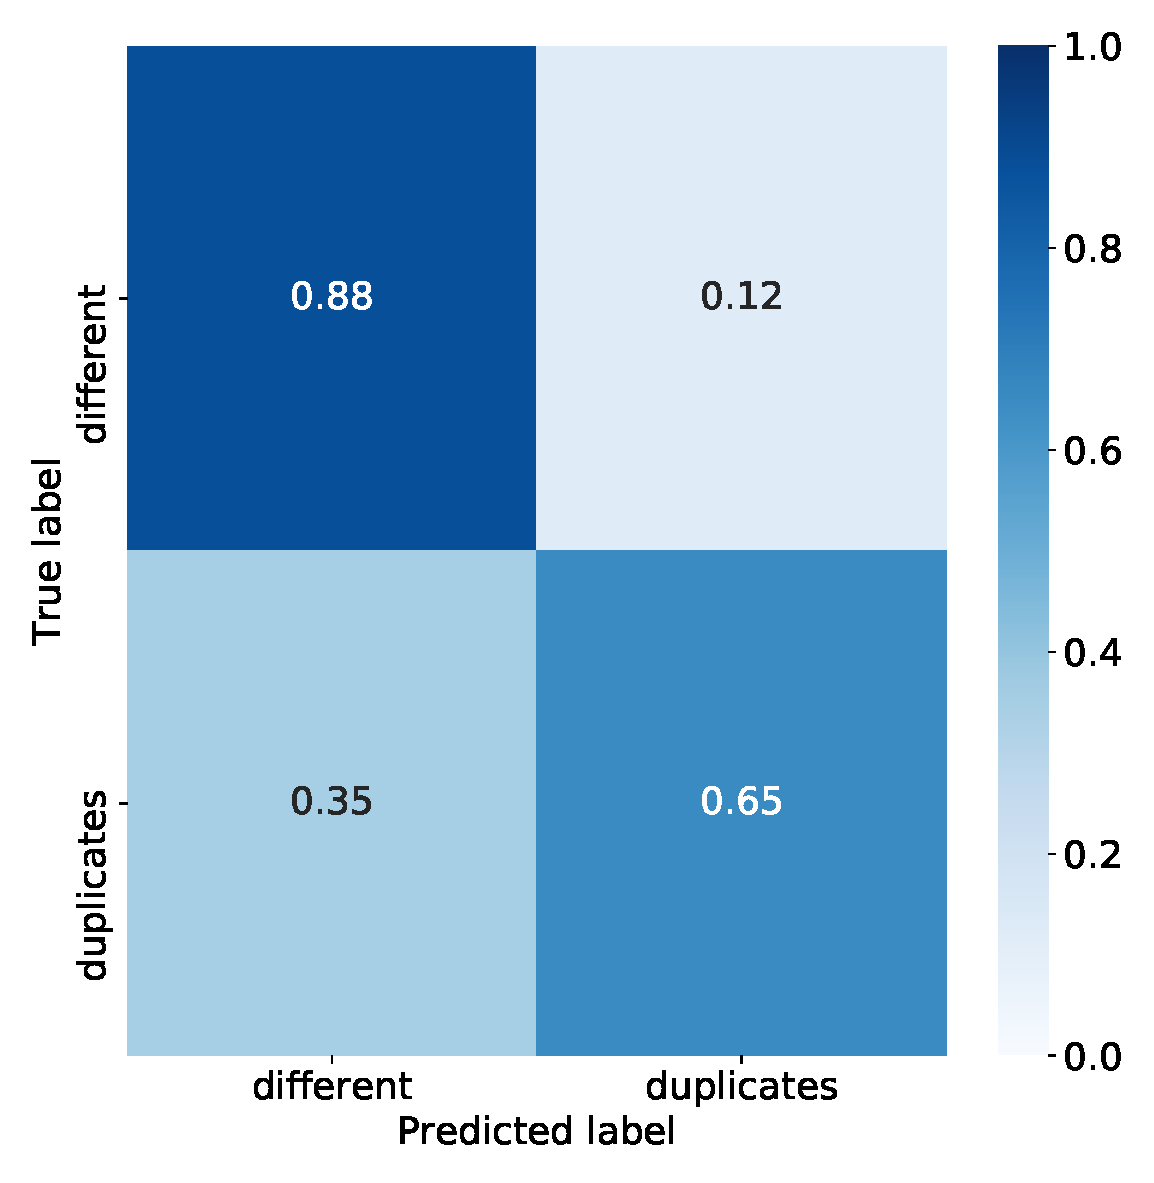
\includegraphics[width=8cm]{BiLSTMCodeEncoder2Cls_conf_mat.eps}
	\centering
	\caption{A confusion matrix for the two-class variant of the BiLSTM code encoder model on a test dataset split.}
	\label{bi_lstm_code_encoder_2cls_conf_mat}
\end{figure}

\begin{figure}[!h]
	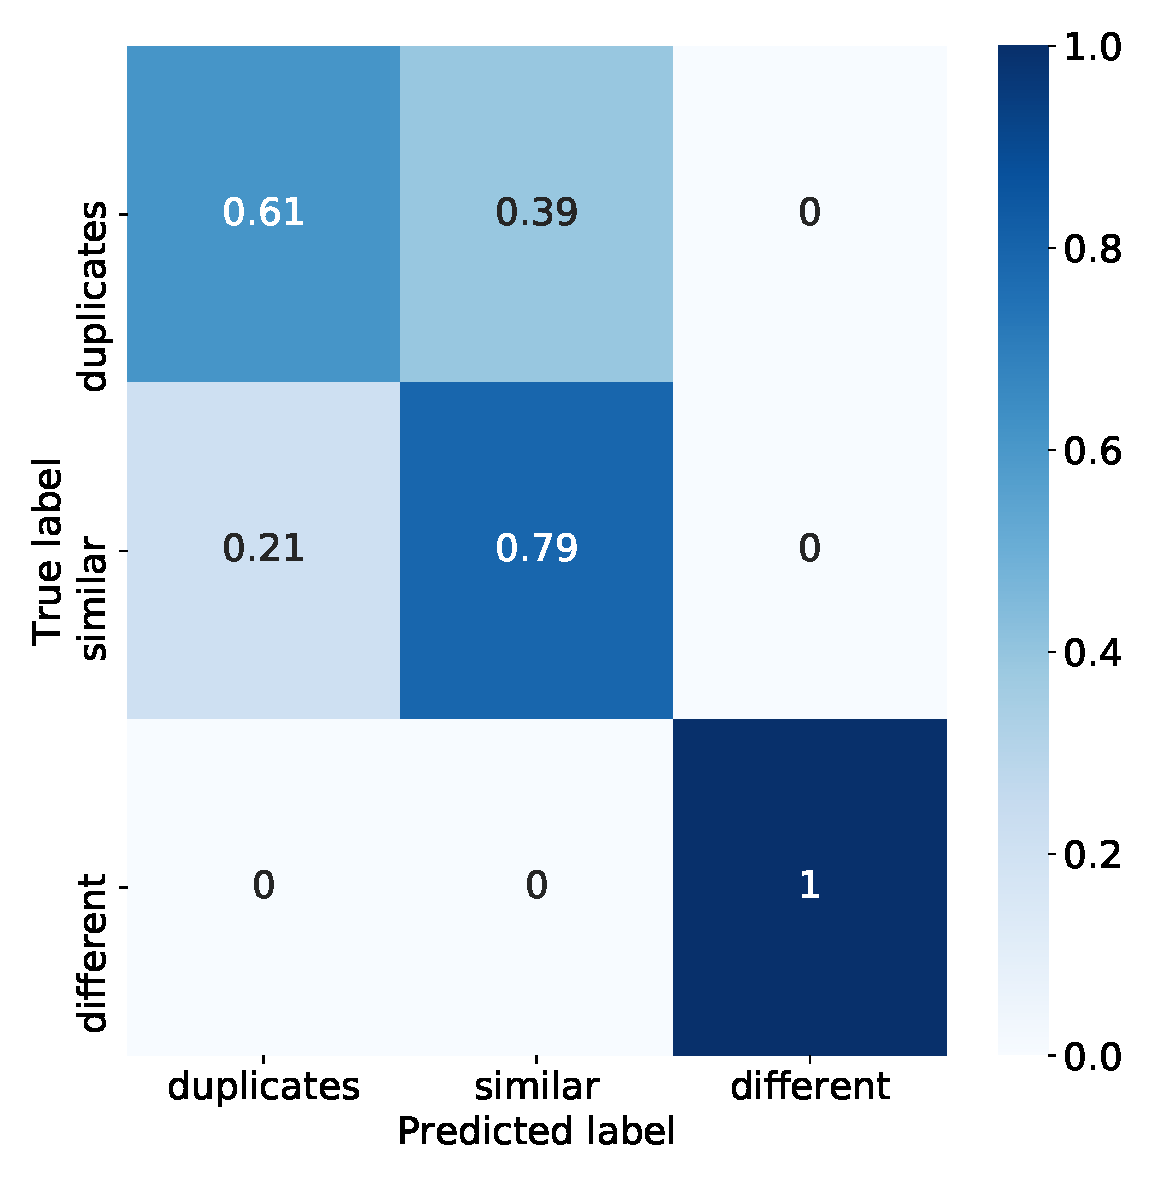
\includegraphics[width=8cm]{BiLSTMCodeEncoder3Cls_conf_mat.eps}
	\centering
	\caption{A confusion matrix for the three-class variant of the BiLSTM code encoder model on a test dataset split.}
	\label{bi_lstm_code_encoder_3cls_conf_mat}
\end{figure}

\subsection{Other experiments}
\paragraph{}
Developing and fine-tuning the model requires a lot of experiments and testing of various techniques. In this work, these are mainly a different loss function and a different merging step. This section briefly discussed the results and conclusions of these experiments.

\paragraph{}
An originally used loss function was a cross-entropy, which correlates very well with accuracy. Unfortunately, with the cross-entropy loss function, the models tend to learn a strong bias towards more numerous classes such as \textit{similar} or \textit{different}, not classifying the \textit{duplicate} examples correctly. To address this problem, the f1 loss function is used instead and it brings a significant improvement observed in both the f1 score and confusion matrix. The improvement of the f1 score achieved by using the f1 loss is around $2\%$ on average.

\paragraph{}
Additionally, the work also investigated the possibility of using the absolute value of an element-wise subtraction as a way of merging the sentence representations. However, this merging technique turns out not to be working very well. As a matter of fact, the absolute difference worsens the f1 score by about $4\%$.

\subsection{Comparison to SNLI}
\paragraph{}
Classification on the SNLI dataset is, to some extent, similar to the task of recognizing duplicate questions. At least the proposed three-class architectures, except the BiLSTM code encoders, apply to this task, which is why the SNLI dataset has been used to verify the proposed models.

\paragraph{}
Since the SNLI dataset does not contain any code, the only models used for the verification on the SNLI are the word summation and BiLSTM encoder models. The results of these models (table \ref{models_vs_snli}) without any architectural change are significantly lower than those presented in \cite{snli} with similar models. However, this is expected since the models proposed in this work are tailored and fine-tuned to a slightly different task and the main aim of this work is to optimize the results for the Stackoverflow dataset, not for the SNLI.

\begin{table}
	\centering
	\begin{tabular}{lr} 
		\hline
		\textbf{Model}          & \multicolumn{1}{l}{\textbf{Test accuracy}}  \\ 
		\hline\hline
		LSTM RNN \cite{snli}    & 77.6                              \\
		Sum of words \cite{snli}& 75.3                              \\
		BiDirLSTM2L3Cls        & 72.1                               \\
		WordSum3Cls            & 69.7                               \\
		\hline
	\end{tabular}
	\caption{An accuracy comparison of the proposed models with the work \cite{snli} on the SNLI dataset.}
	\label{models_vs_snli}
\end{table}


\section{Manual Analysis of Dataset and Errors}\label{analysis_of_dataset_and_errors}
\paragraph{}
The previous section of this chapter states the results we achieved using the proposed models. However, the measured metrics,  such as the f1 score and confusion matrix, heavily depend on having the dataset labeled precisely. In our case, the dataset is extracted from a public webpage with millions of users, and therefore, it can be expected that the dataset may be subject to many errors. More precisely, we assume that some amount of duplicate links may be erroneous. Therefore, we create a manual survey of a subset of question pairs, which shall provide us more profound insights into the achieved results.

\paragraph{}
The subset of question pairs to be analyzed is made up of 100 samples. The first 50 of them are randomly sampled from the dataset examples labeled as \textit{duplicate}. Next 25 samples are chosen from duplicate pairs that are erroneously classified as \textit{different} (type I error) by our \textit{BiLSTM Code Encoder} model. Finally, the remaining 25 samples are chosen from non-duplicate pairs of questions, erroneously classified as \textit{duplicate} (type II error).

\paragraph{}
For each of the survey samples, we asked three independent people who work or study in the information technologies field, to asses whether the questions are duplicates or not. To determine the resulting class for each of the pairs, we choose the predominant answer (answer with two or three votes).

\paragraph{}
The results of the survey are summarized in table \ref{manual_surver_results}. The manual analysis shows that the dataset comprises a not negligible amount of redundant duplicate links. This can heavily affect the results obtained by the neural network and therefore, this shall be considered when evaluating the results. For a detailed listing of respondent answers, see appendix \ref{manual_analysis}.

\smallskip{}
\begin{table}[!h]
	\centering
	\begin{tabular}{l c c c} 
		\hline
		\textbf{Survey subset} & \textbf{Samples total} & \textbf{Duplicates \#} & \textbf{Duplicate \%}  \\ 
		\hline\hline
		random duplicates & 50 & 36 & 72\% \\
		type I error      & 25 & 13 & 52\% \\
		type II error     & 25 & 3  & 12\% \\
		\hline
	\end{tabular}
	\caption{Results of manual survey of the dataset samples. The samples are divided into three categories based on the how they are chosen for the survey.}
	\label{manual_surver_results}
\end{table}


\section{Results Discussion}
\paragraph{}
%- why the f1-score is not too high\\
%- a tendency to mar non-duplicates as duplicates \\
%- some queried similar questions can be duplicated \\
%- a lot of duplicates may not be marked as a duplicate\\
This section builds on the results presented in the previous sections, discussing in more detail why the models can detect at most 65\% of the duplicates. The discussion is mainly from the source data point of view since it can play a significant role in the achieved f1 score. 

%- a tendency to mark non-duplicates as duplicates
\paragraph{}
A first phenomenon that can be observed on the Stackoverflow website is that users often mark questions as duplicates, although the questions focus on slightly different topics. Therefore, the data source contains a not negligible amount of false-positive examples, which have a negative consequence on the network's metrics. We substantiate this statement by manual analysis of the dataset samples (section \ref{analysis_of_dataset_and_errors}), which shows that the proportion of false-positive samples in the dataset is around one quarter.

\paragraph{}
Furthermore, the manual analysis shows that among the dataset examples labeled as \textit{duplicate} but classified as \textit{different} is roughly 48\% of false-positives. If we consider this fact, we get 81\% precision on the duplicate questions, which is a significant improvement over the measured 65\%.

\paragraph{}
Unlike the false-positives, the false-negative examples are not so abundant among the \textit{different} pairs classified as \textit{duplicate} since they make up only 12\% of the errors. Taking this into consideration, we get 89\% precision on the non-duplicate questions. A cause of the false-negative examples is the dataset assembly algorithm (section \ref{assembling_the_dataset}). It is because the dataset shall contain semi-positive samples that are collected by Elasticsearch's full-text queries, which may find unmarked duplicated questions.

\paragraph{}
Based on the manual analysis of errors, we create an estimation of a confusion matrix showing the network results not being affected by errors in the evaluation data. The resulting confusion matrix is depicted in figure \ref{bi_lstm_code_encoder_2cls_conf_mat_correction}. However, it shall be further noted that the accuracy of the network might increase if being trained on data free from such errors.


\paragraph{}
\begin{figure}[!h]
	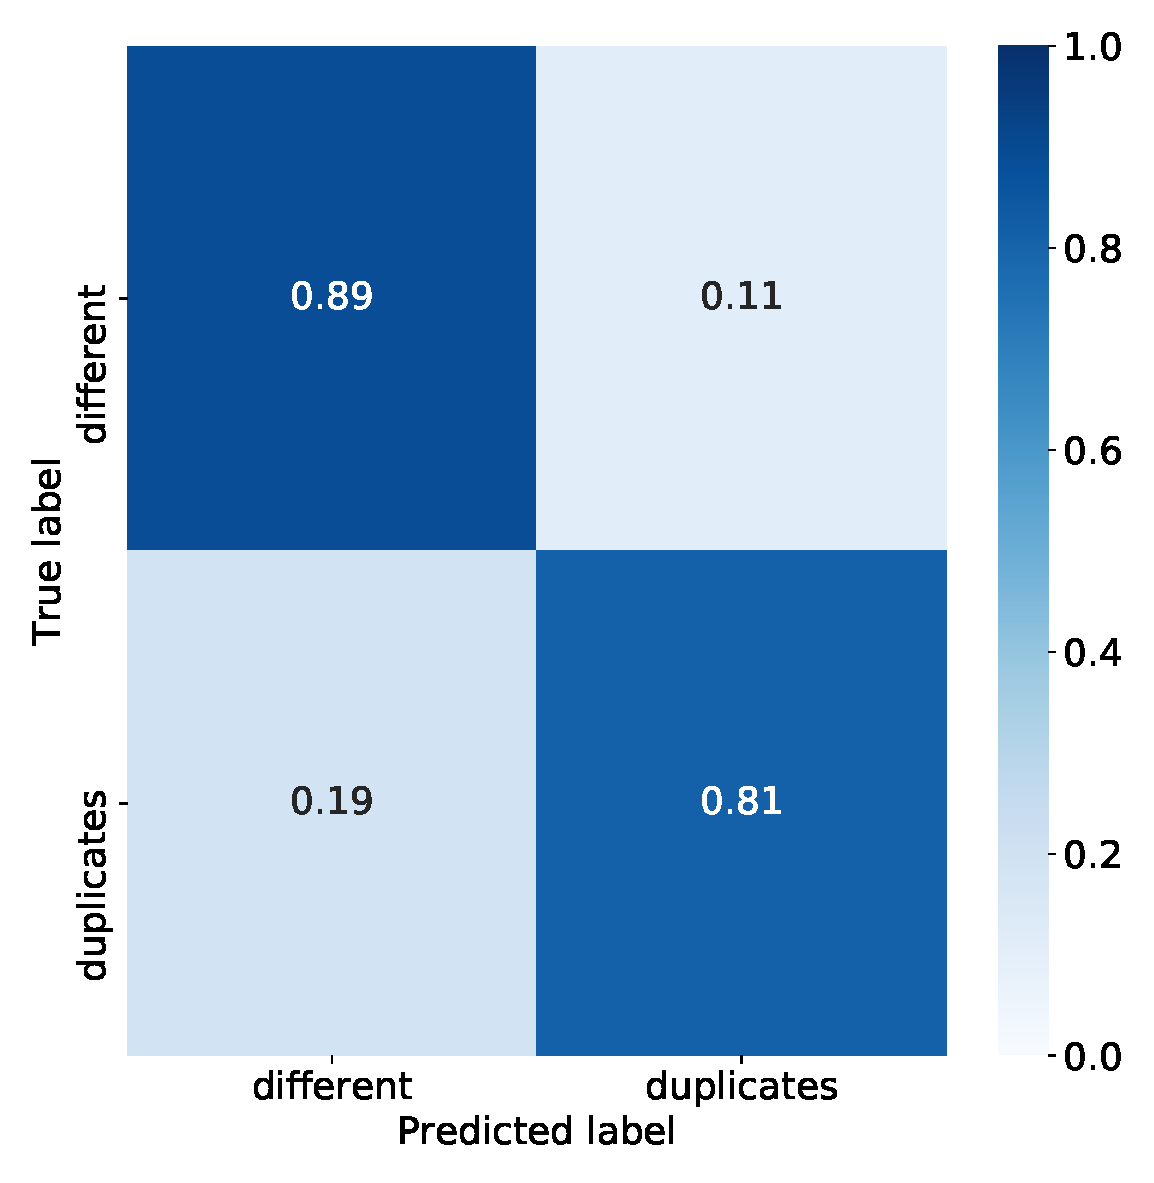
\includegraphics[width=8cm]{BiLSTMCodeEncoder2Cls_conf_mat_correction.eps}
	\centering
	\caption{Resulting confusion matirx of BiLSTM Code Encoder model after correction based on manual error analysis.}
	\label{bi_lstm_code_encoder_2cls_conf_mat_correction}
\end{figure}
